\documentclass[twoside]{book}

% Packages required by doxygen
\usepackage{fixltx2e}
\usepackage{calc}
\usepackage{doxygen}
\usepackage[export]{adjustbox} % also loads graphicx
\usepackage{graphicx}
\usepackage[utf8]{inputenc}
\usepackage{makeidx}
\usepackage{multicol}
\usepackage{multirow}
\PassOptionsToPackage{warn}{textcomp}
\usepackage{textcomp}
\usepackage[nointegrals]{wasysym}
\usepackage[table]{xcolor}

% Font selection
\usepackage[T1]{fontenc}
\usepackage[scaled=.90]{helvet}
\usepackage{courier}
\usepackage{amssymb}
\usepackage{sectsty}
\renewcommand{\familydefault}{\sfdefault}
\allsectionsfont{%
  \fontseries{bc}\selectfont%
  \color{darkgray}%
}
\renewcommand{\DoxyLabelFont}{%
  \fontseries{bc}\selectfont%
  \color{darkgray}%
}
\newcommand{\+}{\discretionary{\mbox{\scriptsize$\hookleftarrow$}}{}{}}

% Page & text layout
\usepackage{geometry}
\geometry{%
  a4paper,%
  top=2.5cm,%
  bottom=2.5cm,%
  left=2.5cm,%
  right=2.5cm%
}
\tolerance=750
\hfuzz=15pt
\hbadness=750
\setlength{\emergencystretch}{15pt}
\setlength{\parindent}{0cm}
\setlength{\parskip}{3ex plus 2ex minus 2ex}
\makeatletter
\renewcommand{\paragraph}{%
  \@startsection{paragraph}{4}{0ex}{-1.0ex}{1.0ex}{%
    \normalfont\normalsize\bfseries\SS@parafont%
  }%
}
\renewcommand{\subparagraph}{%
  \@startsection{subparagraph}{5}{0ex}{-1.0ex}{1.0ex}{%
    \normalfont\normalsize\bfseries\SS@subparafont%
  }%
}
\makeatother

% Headers & footers
\usepackage{fancyhdr}
\pagestyle{fancyplain}
\fancyhead[LE]{\fancyplain{}{\bfseries\thepage}}
\fancyhead[CE]{\fancyplain{}{}}
\fancyhead[RE]{\fancyplain{}{\bfseries\leftmark}}
\fancyhead[LO]{\fancyplain{}{\bfseries\rightmark}}
\fancyhead[CO]{\fancyplain{}{}}
\fancyhead[RO]{\fancyplain{}{\bfseries\thepage}}
\fancyfoot[LE]{\fancyplain{}{}}
\fancyfoot[CE]{\fancyplain{}{}}
\fancyfoot[RE]{\fancyplain{}{\bfseries\scriptsize Generated by Doxygen }}
\fancyfoot[LO]{\fancyplain{}{\bfseries\scriptsize Generated by Doxygen }}
\fancyfoot[CO]{\fancyplain{}{}}
\fancyfoot[RO]{\fancyplain{}{}}
\renewcommand{\footrulewidth}{0.4pt}
\renewcommand{\chaptermark}[1]{%
  \markboth{#1}{}%
}
\renewcommand{\sectionmark}[1]{%
  \markright{\thesection\ #1}%
}

% Indices & bibliography
\usepackage{natbib}
\usepackage[titles]{tocloft}
\setcounter{tocdepth}{3}
\setcounter{secnumdepth}{5}
\makeindex

% Hyperlinks (required, but should be loaded last)
\usepackage{ifpdf}
\ifpdf
  \usepackage[pdftex,pagebackref=true]{hyperref}
\else
  \usepackage[ps2pdf,pagebackref=true]{hyperref}
\fi
\hypersetup{%
  colorlinks=true,%
  linkcolor=blue,%
  citecolor=blue,%
  unicode%
}

% Custom commands
\newcommand{\clearemptydoublepage}{%
  \newpage{\pagestyle{empty}\cleardoublepage}%
}

\usepackage{caption}
\captionsetup{labelsep=space,justification=centering,font={bf},singlelinecheck=off,skip=4pt,position=top}

%===== C O N T E N T S =====

\begin{document}

% Titlepage & ToC
\hypersetup{pageanchor=false,
             bookmarksnumbered=true,
             pdfencoding=unicode
            }
\pagenumbering{roman}
\begin{titlepage}
\vspace*{7cm}
\begin{center}%
{\Large T\+P\+C02 }\\
\vspace*{1cm}
{\large Generated by Doxygen 1.8.11}\\
\end{center}
\end{titlepage}
\clearemptydoublepage
\tableofcontents
\clearemptydoublepage
\pagenumbering{arabic}
\hypersetup{pageanchor=true}

%--- Begin generated contents ---
\chapter{Trabajo Práctico de Clase N°2 -\/ Control de Flujo}
\label{index}\hypertarget{index}{}\hypertarget{index_Files}{}\section{Files}\label{index_Files}

\begin{DoxyItemize}
\item En esta pestaña se encuntra el listado de los archivos referidos al T\+PC \begin{DoxyNote}{Note}
Para correr el programa debe compilarse con el comando make en consola. Luego correr con el comando\+: ./\+T\+P\+C02 
\end{DoxyNote}
\begin{DoxyAuthor}{Author}
Sebastian A. Vega 
\end{DoxyAuthor}
\begin{DoxyVersion}{Version}
1.\+0 
\end{DoxyVersion}

\end{DoxyItemize}
\chapter{File Index}
\section{File List}
Here is a list of all documented files with brief descriptions\+:\begin{DoxyCompactList}
\item\contentsline{section}{\hyperlink{TPC03__1_8c}{T\+P\+C03\+\_\+1.\+c} \\*Primer programa documentado -\/ Info I }{\pageref{TPC03__1_8c}}{}
\end{DoxyCompactList}

\chapter{File Documentation}
\hypertarget{mainTPC02_8c}{}\section{main\+T\+P\+C02.\+c File Reference}
\label{mainTPC02_8c}\index{main\+T\+P\+C02.\+c@{main\+T\+P\+C02.\+c}}


Funcion principal\+: recibira los datos ingresados por el usuario.  


{\ttfamily \#include $<$stdio.\+h$>$}\\*
{\ttfamily \#include $<$stdlib.\+h$>$}\\*
{\ttfamily \#include \char`\"{}T\+P\+C02.\+h\char`\"{}}\\*
Include dependency graph for main\+T\+P\+C02.\+c\+:\nopagebreak
\begin{figure}[H]
\begin{center}
\leavevmode
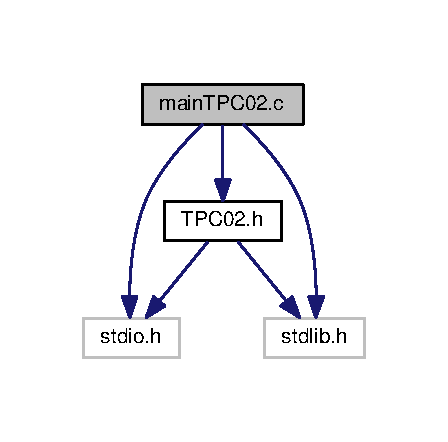
\includegraphics[width=215pt]{mainTPC02_8c__incl}
\end{center}
\end{figure}
\subsection*{Functions}
\begin{DoxyCompactItemize}
\item 
int {\bfseries main} ()\hypertarget{mainTPC02_8c_ae66f6b31b5ad750f1fe042a706a4e3d4}{}\label{mainTPC02_8c_ae66f6b31b5ad750f1fe042a706a4e3d4}

\end{DoxyCompactItemize}


\subsection{Detailed Description}
Funcion principal\+: recibira los datos ingresados por el usuario. 


\hypertarget{TPC02_8h}{}\section{T\+P\+C02.\+h File Reference}
\label{TPC02_8h}\index{T\+P\+C02.\+h@{T\+P\+C02.\+h}}


Archivo Cabecera\+: Tiene los prototipos de función para cada ejercico.  


{\ttfamily \#include $<$stdio.\+h$>$}\\*
{\ttfamily \#include $<$stdlib.\+h$>$}\\*
Include dependency graph for T\+P\+C02.\+h\+:\nopagebreak
\begin{figure}[H]
\begin{center}
\leavevmode
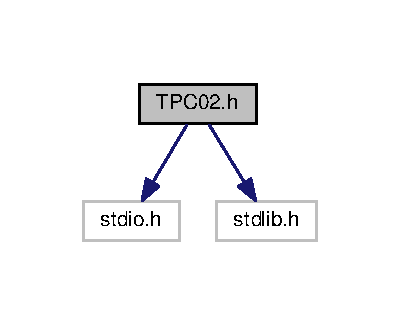
\includegraphics[width=192pt]{TPC02_8h__incl}
\end{center}
\end{figure}
This graph shows which files directly or indirectly include this file\+:\nopagebreak
\begin{figure}[H]
\begin{center}
\leavevmode
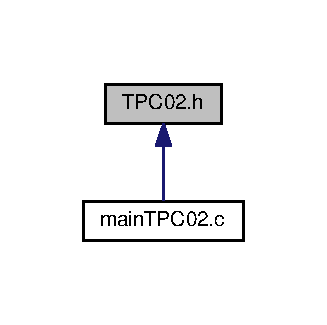
\includegraphics[width=157pt]{TPC02_8h__dep__incl}
\end{center}
\end{figure}
\subsection*{Functions}
\begin{DoxyCompactItemize}
\item 
int {\bfseries compara} (int, int)\hypertarget{TPC02_8h_ad3a662bab001fdfee37469c7f52ba793}{}\label{TPC02_8h_ad3a662bab001fdfee37469c7f52ba793}

\item 
int {\bfseries compara\+\_\+ternario} (int, int)\hypertarget{TPC02_8h_a70fec8c006bfc9014892ccec35d0f868}{}\label{TPC02_8h_a70fec8c006bfc9014892ccec35d0f868}

\item 
int {\bfseries cmp} (int, int, int)\hypertarget{TPC02_8h_aab251a9f927f2e2dc3c27f3fa5c4b69d}{}\label{TPC02_8h_aab251a9f927f2e2dc3c27f3fa5c4b69d}

\item 
int {\bfseries color\+\_\+opc} (int)\hypertarget{TPC02_8h_a1b0c8818be19a7d095c2e94a0c7e7a23}{}\label{TPC02_8h_a1b0c8818be19a7d095c2e94a0c7e7a23}

\item 
int {\bfseries func\+\_\+arr} (int arr\mbox{[}$\,$\mbox{]})\hypertarget{TPC02_8h_a0aa6a2601366f74b4a3000c281b1f4b9}{}\label{TPC02_8h_a0aa6a2601366f74b4a3000c281b1f4b9}

\end{DoxyCompactItemize}


\subsection{Detailed Description}
Archivo Cabecera\+: Tiene los prototipos de función para cada ejercico. 

\begin{DoxyAuthor}{Author}
Sebastian A. Vega 
\end{DoxyAuthor}

\hypertarget{TPC02__1a_8c}{}\section{T\+P\+C02\+\_\+1a.\+c File Reference}
\label{TPC02__1a_8c}\index{T\+P\+C02\+\_\+1a.\+c@{T\+P\+C02\+\_\+1a.\+c}}


determinara cual es mayor de los números ingresados  


{\ttfamily \#include $<$stdio.\+h$>$}\\*
{\ttfamily \#include $<$stdlib.\+h$>$}\\*
Include dependency graph for T\+P\+C02\+\_\+1a.\+c\+:\nopagebreak
\begin{figure}[H]
\begin{center}
\leavevmode
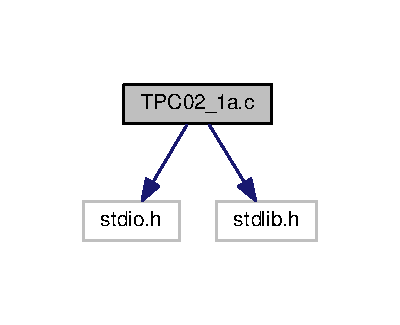
\includegraphics[width=192pt]{TPC02__1a_8c__incl}
\end{center}
\end{figure}
\subsection*{Functions}
\begin{DoxyCompactItemize}
\item 
int {\bfseries compara} (int a, int b)\hypertarget{TPC02__1a_8c_a1fb4cfdcfd69b0133beb3e0775991898}{}\label{TPC02__1a_8c_a1fb4cfdcfd69b0133beb3e0775991898}

\end{DoxyCompactItemize}


\subsection{Detailed Description}
determinara cual es mayor de los números ingresados 

Ejercicio\+: Realizar una función que reciba dos números e imprima el mayor de ellos (si son iguales puede imprimir cualquiera de los dos) \begin{DoxyNote}{Note}
esto también es para evaluar el comportamiento de Doxygen 
\end{DoxyNote}

\begin{DoxyParams}{Parameters}
{\em a,b} & \\
\hline
\end{DoxyParams}
\begin{DoxyAuthor}{Author}
Sebastian A. Vega 
\end{DoxyAuthor}

%--- End generated contents ---

% Index
\backmatter
\newpage
\phantomsection
\clearemptydoublepage
\addcontentsline{toc}{chapter}{Index}
\printindex

\end{document}
